% The per-edge policy head (fig:edgescore, eq:edgescore in 4.Implementation.tex).
% Build:  latexmk -pdf edgescore.tex  -> edgescore.pdf, copy to Images/.
% Fonts match the thesis (lmodern + T1).
\documentclass[border=3pt]{standalone}
\usepackage{lmodern}
\usepackage[T1]{fontenc}
\usepackage{amsmath}
\usepackage{tikz}
\usetikzlibrary{positioning,arrows.meta,calc,decorations.pathreplacing,fit,backgrounds}

% Palette shared with base.py (C dict).
\definecolor{storeF}{HTML}{CFE3F7}
\definecolor{ctrlF}{HTML}{D7F0D8}
\definecolor{estF}{HTML}{F7D6D6}
\definecolor{taskF}{HTML}{F6E7C1}
\definecolor{ink}{HTML}{43505C}
\definecolor{accent}{HTML}{2F6FAE}
\definecolor{agent}{HTML}{C0392B}
\definecolor{muted}{HTML}{5A6673}

\tikzset{
  v/.style={circle, draw=ink, fill=white, minimum size=8mm, inner sep=0pt, line width=0.8pt},
  ag/.style={circle, fill=agent, minimum size=4.2mm, inner sep=0pt},
  edge/.style={-{Stealth[length=2.4mm]}, line width=1.1pt, draw=accent},
  box/.style={draw=ink, line width=0.8pt, rounded corners=3pt, align=center,
              font=\small, inner sep=4pt, minimum height=9mm},
  flow/.style={-{Stealth[length=2.2mm]}, line width=0.8pt, draw=ink},
  lbl/.style={font=\footnotesize, text=muted},
}

\begin{document}
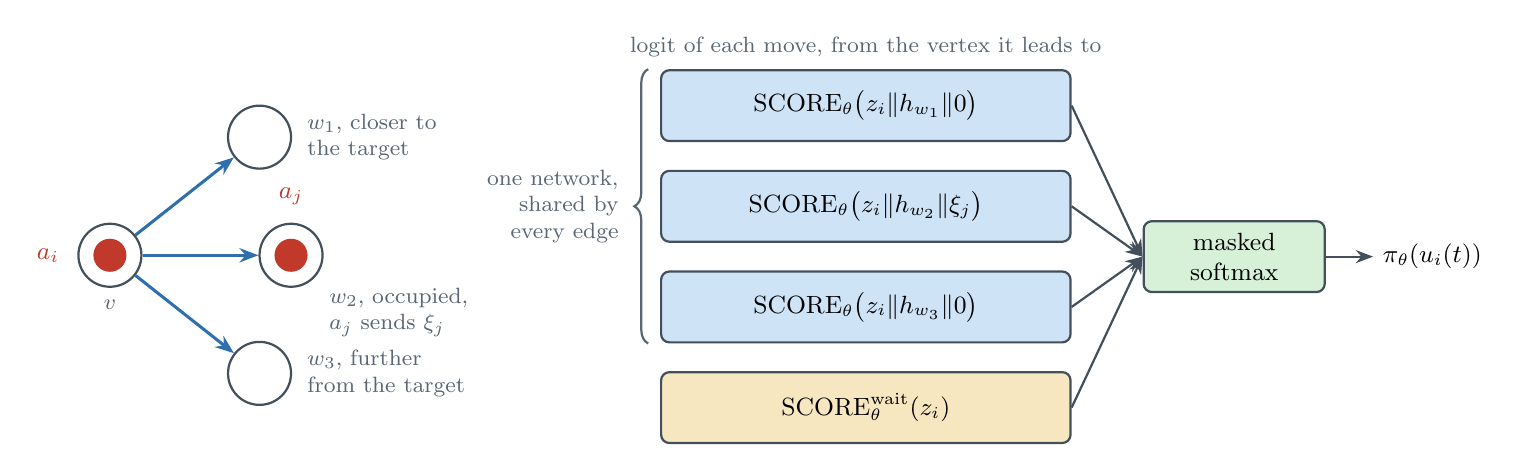
\begin{tikzpicture}
  % ------------------------------------------------ the agent's neighbourhood
  \node[v] (v) at (0,0) {};
  \node[ag] at (v) {};
  \node[font=\small, text=agent, left=3pt of v] {$a_i$};
  \node[lbl, below=1pt of v] {$v$};

  \node[v] (w1) at (1.9, 1.5) {};
  \node[v] (w2) at (2.3, 0) {};
  \node[v] (w3) at (1.9,-1.5) {};
  \node[ag] at (w2) {};
  \node[font=\small, text=agent, above=3pt of w2] {$a_j$};

  \draw[edge] (v) -- (w1);
  \draw[edge] (v) -- (w2);
  \draw[edge] (v) -- (w3);

  \node[lbl, right=2pt of w1, align=left] {$w_1$, closer to\\ the target};
  \node[lbl, below right=0pt and 2pt of w2, align=left] {$w_2$, occupied,\\ $a_j$ sends $\xi_j$};
  \node[lbl, right=2pt of w3, align=left] {$w_3$, further\\ from the target};

  % ------------------------------------------------ one score per edge
  \node[box, fill=storeF, minimum width=5.2cm] (s1) at (9.6, 1.9)
    {$\mathrm{SCORE}_\theta\bigl(z_i \Vert h_{w_1} \Vert 0\bigr)$};
  \node[box, fill=storeF, minimum width=5.2cm, below=0.35cm of s1] (s2)
    {$\mathrm{SCORE}_\theta\bigl(z_i \Vert h_{w_2} \Vert \xi_j\bigr)$};
  \node[box, fill=storeF, minimum width=5.2cm, below=0.35cm of s2] (s3)
    {$\mathrm{SCORE}_\theta\bigl(z_i \Vert h_{w_3} \Vert 0\bigr)$};
  \node[box, fill=taskF, minimum width=5.2cm, below=0.35cm of s3] (sw)
    {$\mathrm{SCORE}^{\mathrm{wait}}_\theta(z_i)$};

  \draw[decorate, decoration={brace, amplitude=5pt, mirror}, line width=0.8pt, draw=muted]
    ($(s1.north west)+(-0.15,0)$) -- ($(s3.south west)+(-0.15,0)$)
    node[midway, left=7pt, lbl, align=right] {one network,\\ shared by\\ every edge};

  % ------------------------------------------------ softmax and choice
  \node[box, fill=ctrlF, right=0.9cm of $(s2.east)!0.5!(s3.east)$, minimum width=2.3cm] (sm)
    {masked\\ softmax};
  \node[font=\small, right=0.6cm of sm] (pi) {$\pi_\theta(u_i(t))$};

  \foreach \s/\l in {s1/{move to $w_1$}, s2/{move to $w_2$}, s3/{move to $w_3$}, sw/{wait}} {
    \draw[flow] (\s.east) -- (sm.west);
  }
  \draw[flow] (sm) -- (pi);

  \node[lbl, above=1pt of s1] {logit of each move, from the vertex it leads to};
\end{tikzpicture}
\end{document}
